\documentclass{article}

% ready for submission
\usepackage[preprint, nonatbib]{nips_2018}
\bibliographystyle{abbrvnat}

\usepackage[utf8]{inputenc} % allow utf-8 input
\usepackage[T1]{fontenc}    % use 8-bit T1 fonts
\usepackage[hidelinks]{hyperref}       % hyperlinks
\usepackage{url}            % simple URL typesetting
\usepackage{booktabs}       % professional-quality tables
\usepackage{amsfonts}       % blackboard math symbols
\usepackage{nicefrac}       % compact symbols for 1/2, etc.
\usepackage{microtype}      % microtypography
\usepackage{graphicx}
\usepackage{tabularx}
\usepackage{ctex}
\usepackage{multirow}
\usepackage{amsmath}
\usepackage{bookmark}
\usepackage{float}
\usepackage{subcaption}    
\usepackage{authblk}
\usepackage{amssymb}
\usepackage{pdfpages}
\setlength{\parindent}{2em} % 全局缩进设为 2em

\let\oldcite\cite
\renewcommand{\cite}[1]{\oldcite{#1}}

\title{大直径钢管直度测量系统设计方案}

\renewcommand*{\Authands}{，}     % 多个作者时，最后两个作者之间的连接符
\author{陈昭宇}
\author{梁炎明\thanks{Email: liangym@xaut.edu.cn}}
\author{张耀阳}
\author{俞超翔}
\author{王玥}
\author{白星宇}

% 定义单位
\affil{西安理工大学}

\begin{document}

% \includepdf[pages=8]{abab.pdf}

\maketitle

\begin{abstract}
	测量钢管直度是钢管生产过程中重要的质量控制环节。传统接触式方法效率低、易划伤表面；现有非接触式方案测量范围有限，
    且难以消除钢管运动过程中震动与偏移引入的系统误差。
	本文提出一种基于双RGBD相机点云数据的大直径钢管直度在线测量算法。该算法通过点云拼接与预处理获取高质量钢管局部点云，
    利用PCA估计轴线方向并进行切片，采用RANSAC粗拟合结合非线性最小二乘细拟合确定各截面圆心坐标，
    并通过二阶差分法消除传感器安装误差与钢管刚体运动引入的旋转平移误差，有效抑制钢管轴向进给过程中位移抖动对测量精度的影响。
    在此基础上，利用分Bin平均降低随机测量噪声，再经加权PCA降维与两次数值积分重建钢管轴线偏差曲线，最终计算直度。
    我们搭建了基于铝型材框架与伺服电机直线模组的微缩测试平台，验证了点云分割算法的有效性，为后续算法验证提供了稳定的数据来源。
    本文相关代码已开源，见 \url{https://github.com/ZiYuLab/tube_straightness_measure}。
\end{abstract}

\section{引言}

钢管直线度测量作为工业质量控制中的重要环节，其精度对后续加工工艺和最终产品性能具有深远影响。无缝钢管凭借其卓越的力学性能和耐腐蚀性，
在石油天然气输送、航空航天以及汽车零部件制造等领域得到了广泛应用。然而，钢管的直线度偏差可能会带来一系列问题，例如装配困难、
应力集中或流体阻力增加等，这些问题不仅会降低产品的可靠性，还可能缩短其使用寿命。

目前已知国内外钢管直度检测方法主要分为两大类，分别是接触式测量和非接触测量。
传统方法中，采用拉线法与直尺法，工人通过拉线或直尺直接接触钢管表面，肉眼判断直线度偏差。
其优点是操作简单、成本低，但效率低下且精度受主观因素影响，难以满足大规模生产需求。
使用三坐标测量机对钢管进行多点接触式测量，精度较高，但需逐点检测，耗时较长，且设备昂贵，仅适用于实验室或小批量抽检场景。
部分生产线通过校直机的机械接触反馈间接判断直线度，但这类方法需依赖后续加工效果，无法实现实时检测，且可能因过度校直损伤钢管。
接触式方法普遍存在效率低、易划伤表面、无法在线检测等问题，尤其不适用于高温或高速生产线。
非接触式方法具有高效、无损伤、实时性强等特点。
采用激光束或光电传感器扫描钢管表面，通过光信号反射或遮挡分析直线度偏差。例如，通过旋转钢管并配合激光灯头照射，实时捕捉弯曲数据。
此类技术精度可达微米级，且支持高速在线检测，适用于工业现场。
利用光学原理检测钢管的微小角度偏差，结合算法转换为直线度数据。此类方法精度高，但对环境稳定性要求较高，多用于精密仪器校准或实验室环境。
当前主流发展方向集中于激光、光电和视觉检测技术的优化，以实现在线、实时、高精度的综合检测需求。
非接触式检测设备正与工业物联网（IIoT）融合，实现检测数据实时分析及工艺优化反馈，推动质量控制的闭环管理。如激光与视觉技术的结合，
可兼顾高速与高精度检测需求。随着传感器技术发展，非接触式设备的成本逐步降低，未来有望在中小型企业普及。

早在2001年便有研究提出一种基于机器视觉的钢管直度检测方案\cite{cv}，然而该方案受限于视觉传感器的像素精度。
2002年Wei Gao团队提出了一种使用三对单点激光测距进行钢管直度检测的方案，使用了差分积分法能够有效消除由于传感器安装位置导致的误差，
并且提出了一种传感器调零校准的方案\cite{pm}。但是单点测距的范围较小，误差的消除方法也仅适用于二维平面测量，无法处理三维旋转和平移误差。 
2003年，来自天津大学的吴有华等人发明出一款钢管直度测量视觉传感器，采用双光条结构提高圆心定位精度， 优化传感器设计，这种标定方法简单高效，
悬丝法比传统齿形靶标定更方便，精度相当。缺点是容易受到设备限制，标定依赖经纬仪等辅助工具，增加操作复杂度，适用范围较窄，主要针对钢管，
未提及其他形状的适用性。  
2011年，重庆大学的李小涛团队提出了一种基于激光视觉在线测量的方法。该方法通过非接触式多传感器协同工作，
并结合高精度算法实现了无缝钢管直线度的在线检测。这种方法特别适用于大尺寸工件的自动化生产场景，但由于系统复杂且成本较高，
其进一步推广仍需优化以适应更广泛的工业需求。
2017年，由中石化石油工程机械有限公司的黄雄飞等人提出一种钢管制直度测量方法，该研究提出一种基于激光测距和管端识别传感器的直缝钢管直度测量方法，
利用X光检查小车回程自动完成测量。优点是自动化高效，利用现有X光小车回程测量，无需额外作业环节\cite{hxf}; 缺点是精度受限，精度可能无法满足高要求场景。
并且依赖小车速度，适用范围窄，仅针对直缝钢管焊缝方向的弯曲，未涵盖全方位变形检测。
随后，在2018年，南通盛立德金属材料科技有限公司的杭伟发明了一种新的钢管直线度检测器。该设备利用线性弹簧隔振和柔性连轴器技术，
能够适应不同规格钢管的检测需求，展现出较广的应用范围。不过，这一方法仅适用于旋转检测，无法检测静态变形，因此存在一定的局限性。
2021年Kshaurad等人利用了相机并采用了最小区域公差算法用于钢管圆度的测量\cite{cv_yd}；
随后在2023年Andrea Egidi等人采用了一种基于机械调制的激光检测方法来测量钢管直度\cite{tzzxd}，然而该方法仅能测量局部直线度，无法获取全管段的整体弯曲信息。


为降低成本、提升精度，本文提出一种基于双RGBD相机点云数据的大直径钢管直度在线测量算法。该算法以两台Intel D435 RGBD相机采集的点云及传送带位置传感器数据为输入，通过点云拼接与预处理获取高质量钢管局部点云，利用PCA估计轴线方向并进行截面切片，采用RANSAC粗拟合结合非线性最小二乘细拟合确定各截面圆心坐标。通过二阶差分法消除传感器安装误差与钢管刚体运动引入的旋转平移误差，有效抑制钢管轴向进给过程中位移抖动对测量精度的影响。在此基础上，利用分Bin平均降低随机测量噪声，再经加权PCA降维与两次数值积分重建钢管轴线偏差曲线，最终计算直度。我们搭建了基于铝型材框架与伺服电机直线模组的微缩测试平台，验证了点云分割算法的有效性，为后续算法验证提供了稳定的数据来源。

\section{方法}

\subsection{总览}

\begin{figure}[!htb]
    \centering
    
\includegraphics[width=\linewidth]{images/overview.png}
    \caption{系统总览}
    \label{fig:overview}
\end{figure}

系统总览如图\ref{fig:overview}所示。整个系统的传感器部分为两个RGBD相机输出的点云数据（包括其相对于世界坐标的变换），及传送带的位置传感器，用于检测钢管在传送带上的位置。一般情况下，我们只能知道钢管在传送系统（即世界坐标系）的轴线（$x$轴）的位置信息，此处我们仅需要该信息。关于算法部分，接收到的点云通过拼接和预处理，输出仅保留钢管区域的相机可视有效点云数据，然后对这段点云进行去旋转操作，以避免切片投影后的椭圆形2D点云对圆形拟合产生的影响，并随后进行三段点云切片。在圆形拟合部分，我们采用RANSAC粗拟合加最小二乘细拟合方案，以确保在两传感器无法完全覆盖钢管的前提下的圆形拟合精度。紧接着，我们根据位置传感器信息将得到的三段点云切片转换到世界坐标系中，得到圆形的绝对位置，并同时计算圆心处钢管的二阶差分数据（曲率）。在全部钢管扫描完成后，我们可以分bin将数据存入，并计算每bin的各数据均值从而降低噪声对精度的影响。紧接着，我们利用加权PCA得到钢管的主方向和弯曲主方向，将三维问题降低为二维问题，最后对二阶差分数据进行两次积分，从而得到钢管中心在钢管坐标系下的序列，进而得到直度。

\subsection{坐标系定义}

\begin{figure}[!htb]
    \centering
    
\includegraphics[width=0.8\linewidth]{images/frame_def.png}
    \caption{坐标系定义}
    \label{fig:frame_def}
\end{figure}

为了便于描述和计算，我们定义坐标系如图\ref{fig:frame_def}所示，各坐标系解释如下：

\begin{itemize}
    \item RGBD相机坐标系（$R_1$、$R_2$）：$x$轴为相机光轴方向，$y$轴为像平面长边方向。
    \item 世界坐标系（$W$）：$x$为传送带正向，$z$为正向上。
    \item 钢管坐标系（$T$）：$x$轴为钢管两侧圆心连线，与$W$系$x$轴正向呈锐角，$z$轴为正向上。
\end{itemize}

对于以上坐标系，RGBD与世界坐标系的变换可以由手眼标定算法得到，因而为已知量，钢管坐标系与世界坐标系的$x$向平移可由位置传感器得到，其余变换关系均未知。由于钢管坐标系原点与直度无关，因此可以任意选取。

\subsection{点云处理}

\subsubsection{深度感知与点云预处理}

深度图像的精确获取是后续点云配准与直度分析的基础。系统通过 pyrealsense2 API 驱动深度相机集群，获取高分辨率深度流（z16格式）。针对工业现场及机械导轨运动可能引入的高频震动与散斑噪声，系统在三维点云重建前，构建了三级硬件级滤波管线：
\begin{itemize}
\item 降采样滤波 (Decimation Filter)：对原始深度图像进行空间维度的亚采样，在显著降低后续点云计算量的同时，实现局部噪声的平滑抑制。
\item 空间阈值滤波 (Threshold Filter)：结合测试台的物理尺寸与相机安装位姿，设定深度的上下限截断阈值。此步骤可直接在底层剔除观测工作区（ROI）之外的无效背景，大幅提高有效数据占比。
\item 时域滤波 (Temporal Filter)：利用多帧深度图的时间连续性特征，通过历史帧加权平均，对缺失或因反射率问题失效的深度像素进行补偿。
\end{itemize}

由于RGBD与世界坐标系的变换已知，我们可以容易计算点云中的每一点相对于世界坐标系的坐标，从而能够对两传感器的点云数据进行坐标变换和拼接：
\begin{equation}
    {}^W\mathbf{p}_i = {}^W_{R_k}\mathbf{R} \; {}^{R_k}\mathbf{p}_i + {}^W_{R_k}\mathbf{t}
\end{equation}

由于RGBD相机点云密度随深度逐渐下降，其分布不均的特性将会对圆拟合造成麻烦；其次，大量的点云会显著降低处理速度。因此采用对点云进行适当体素下采样的方式来解决以上问题。

\subsubsection{点云分割}

在测试台运行过程中，直接获取的点云包含大量支撑支架、导轨等非目标背景。为获取纯净的钢管表面点云，系统设计了"空间距离背景差分 + DBSCAN密度聚类"的级联分割算法。

在系统初始化阶段，相机采集空载状态（无钢管）下的多帧静止点云，融合构建为基准背景模型 $P_{\text{bg}}$。在动态测量阶段，设当前帧点云为 $P_t$，针对 $P_t$ 中的任意点 $p_i$，计算其到背景模型的最短欧氏距离：
\begin{equation}
    d(p_i, P_{\text{bg}}) = \min_{p_j \in P_{\text{bg}}} \| p_i - p_j \|_2
\end{equation}

引入背景判定阈值 $\tau$（本项目优选为 0.02\,m），通过硬截断提取出疑似钢管的前景点云集合：
\begin{equation}
    P_{\text{fg}} = \{ p_i \in P_t \mid d(p_i, P_{\text{bg}}) > \tau \}
\end{equation}

由于前景中不可避免地掺杂了运动飞溅物或光线变化带来的孤立噪声点，系统对 $P_{\text{fg}}$ 引入DBSCAN算法进行语义级过滤。设定邻域搜索半径 $\epsilon = 0.025$，核心点最小密度阈值 $\text{MinPts} = 30$。算法通过密度可达性判定，将散乱点云连通为独立的聚类簇 $C_k$。最终，提取点数最多的类簇作为高置信度的钢管有效表面点云 $S_{\text{pipe}}$：
\begin{equation}
    S_{\text{pipe}} = \arg\max_{C_k} |C_k|
\end{equation}

\subsection{有效区域轴线方向估计和片段截取}

经上述步骤处理，我们便可以得到质量较高、分布均匀、没有背景物体的钢管局部点云数据。考虑到实际应用中直度多为毫米级，因而此局部点云片段可近似看作标准圆柱体。然而由于钢管在传送系统运送时，局部可能不平行于世界坐标系的$x$轴，因此直接将可见范围点云切分将会得到椭圆形切片，从而降低精度。因此，可以使用PCA方法，找到当前局部点云的真实轴线方向，并以该方向切分点云。

由于RGBD相机的可见局部点云，点沿轴线方向的散布远大于横截面方向的散布，因此最大方差方向必为轴线方向。寻找真实轴线问题转换为寻找一组三维正交基$\{\mathbf{e}_1, \mathbf{e}_2, \mathbf{e}_3\}$使得点云数据在这些正交基上的投影方差依次达到最大，这等价于对局部点云进行主成分分析（PCA）\cite{pca}。

首先对点云去中心化：
\begin{equation}
    \mathbf{q}_i = \mathbf{p}_i - \bar{\mathbf{p}}, \quad \bar{\mathbf{p}} = \frac{1}{n} \sum_{i=1}^n \mathbf{p}_i
\end{equation}

设单位向量 $\mathbf{u}$，点云在 $\mathbf{u}$ 上的投影方差为：
\begin{equation}
    J(\mathbf{u}) = \frac{1}{n} \sum_{i=1}^n (\mathbf{u}^\top \mathbf{q}_i)^2
    = \mathbf{u}^\top \mathbf{C} \mathbf{u}
\end{equation}

其中 $\mathbf{C} = \frac{1}{n} \sum_{i=1}^n \mathbf{q}_i \mathbf{q}_i^\top$ 为点云的协方差矩阵（$3\times3$ 实对称半正定矩阵）。

求解约束优化问题：
\begin{equation}
    \max_{\mathbf{u}} \; \mathbf{u}^\top \mathbf{C} \mathbf{u} \quad \text{s.t.} \quad \mathbf{u}^\top \mathbf{u} = 1
\end{equation}

引入拉格朗日乘子 $\lambda$，对 $\mathbf{u}$ 求梯度并令其为零，可得：
\begin{equation}
    \mathbf{C}\mathbf{u} = \lambda\mathbf{u}
\end{equation}

因此，$\mathbf{u}$ 必为协方差矩阵 $\mathbf{C}$ 的特征向量，$\lambda$ 为对应特征值。记特征值排序 $\lambda_1 \ge \lambda_2 \ge \lambda_3 \ge 0$，对应的单位特征向量为 $\mathbf{e}_1, \mathbf{e}_2, \mathbf{e}_3$，则第一主方向 $\mathbf{e}_1$ 即为所求轴线方向。

基于此，可以得到当前局部坐标系（PCA系）与世界坐标系中点的旋转变换关系：
\begin{equation}
    \mathbf{q}_i' = {}^{PCA}_W R \; \mathbf{q}_i = [\mathbf{e}_1, \mathbf{e}_2, \mathbf{e}_3]^\top \mathbf{q}_i
\end{equation}

以有效范围中心为中心，设定片段厚度和切片步长，以$x'$为轴对有效范围的钢管点云进行切片，从而得到三个点云片段（$i = 1, 2, 3$）和其对应$x'$轴上的片段中心点${}^{PCA}\mathbf{p}_{ci}$的$x'$轴分量，如图\ref{fig:cutting}所示。

\begin{figure}[!htb]
    \centering
    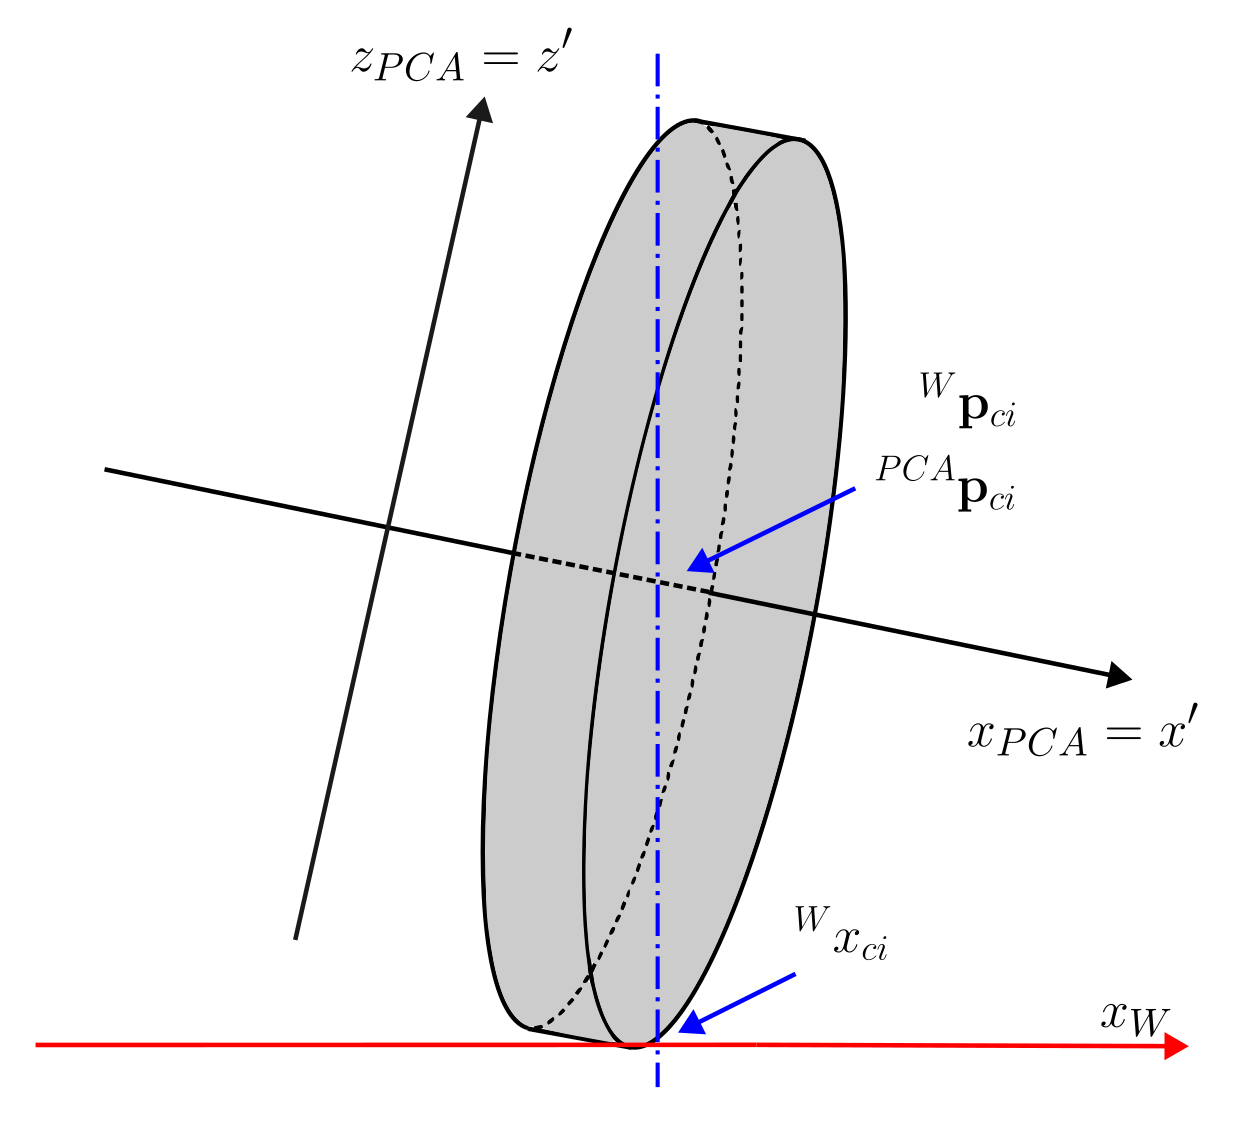
\includegraphics[width=0.8\linewidth]{images/cutting.png}
    \caption{点云切片示意}
    \label{fig:cutting}
\end{figure}

\subsection{轴心坐标点确定}

为计算二阶差分，我们需要分别得到三段点云片段几何中心${}^W\mathbf{p}_{ci}$的坐标。若能得到切割片段几何中心${}^{PCA}\mathbf{p}_{ci}$的坐标，并基于上节得到的旋转矩阵，即可计算得到${}^W\mathbf{p}_{ci}$：
\begin{equation}
    {}^W\mathbf{p}_{ci} = {}^{PCA}_W R^\top \; {}^{PCA}\mathbf{p}_{ci}
\end{equation}

由于切割步长和片段厚度已知，因此可以得到${}^{PCA}\mathbf{p}_{ci}$的$x$分量，于是只需得到其$y$-$z$分量即可，问题简化为一个二维圆形拟合问题。

由于本项目采用双传感器方案，无法得到完整的钢管点云数据，因此考虑先使用RANSAC提供良好初始值并过滤离群点，再建立最小二乘问题进行拟合。

\subsubsection{模型建立}

设去除$x'$分量后的点集，待拟合的圆心和半径为：
\begin{equation}
    \mathbf{p}_i =
    \begin{bmatrix} y_i \\ z_i \end{bmatrix}, \quad
    \mathbf{c} =
    \begin{bmatrix} y_c \\ z_c \end{bmatrix}, \quad r > 0
\end{equation}

每个点到圆的残差定义为：
\begin{equation}
    e_i(\mathbf{c}, r) = \left\| \mathbf{p}_i - \mathbf{c} \right\|_2 - r
\end{equation}

目标是找到使残差尽可能小的圆心与半径：
\begin{equation}
    \min_{\mathbf{c}, r} \sum_{i=1}^{N} e_i(\mathbf{c}, r)^2
\end{equation}

\subsubsection{RANSAC 粗拟合}

RANSAC的作用是从含有离群点的点集中，快速估计一个较可靠的圆初值\cite{ransac}。每次迭代随机选择三个非共线点 $\mathbf{p}_a,\ \mathbf{p}_b,\ \mathbf{p}_c$，三点唯一确定一个候选圆 $\hat{\mathbf{c}},\ \hat{r}$。对所有点计算候选模型残差，若残差小于阈值 $\tau$，则该点被认为是内点：
\begin{equation}
    \hat{e}_i = \left| \left\| \mathbf{p}_i - \hat{\mathbf{c}} \right\|_2 - \hat{r} \right| < \tau
\end{equation}

每次迭代统计内点数量，选择内点数最多的候选圆作为粗拟合结果：
\begin{equation}
    (\mathbf{c}_0, r_0) =
    \arg\max_{(\hat{\mathbf{c}}, \hat{r})}
    \left| \mathcal{I}(\hat{\mathbf{c}}, \hat{r}) \right|
\end{equation}

\subsubsection{最小二乘细拟合}

RANSAC得到初值后，将圆心和半径作为优化变量 $\mathbf{x} = [y_c, z_c, r]^\top$，对所有$M$个点建立残差：
\begin{equation}
    f_i(\mathbf{x}) = \sqrt{(y_i - y_c)^2 + (z_i - z_c)^2} - r
\end{equation}

优化问题为：
\begin{equation}
    \min_{\mathbf{x}} \frac{1}{2} \left\| \mathbf{f}(\mathbf{x}) \right\|_2^2
\end{equation}

在迭代求解中，对当前估计 $\mathbf{x}_k$ 处的残差做一阶线性化：
\begin{equation}
    \mathbf{f}(\mathbf{x}_k + \Delta \mathbf{x}) \approx \mathbf{f}(\mathbf{x}_k) + \mathbf{J}_k \Delta \mathbf{x}
\end{equation}

其中第 $i$ 行雅可比为：
\begin{equation}
    \frac{\partial f_i}{\partial \mathbf{x}} =
    \begin{bmatrix}
    \dfrac{y_c - y_i}{\sqrt{(y_i - y_c)^2 + (z_i - z_c)^2}} &
    \dfrac{z_c - z_i}{\sqrt{(y_i - y_c)^2 + (z_i - z_c)^2}} &
    -1
    \end{bmatrix}
\end{equation}

对应的正规方程为：
\begin{equation}
    \mathbf{J}_k^{\top} \mathbf{J}_k \Delta \mathbf{x} = -\mathbf{J}_k^{\top} \mathbf{f}(\mathbf{x}_k)
\end{equation}

采用ceres-solver求解上述问题，优化收敛后得到最终圆心 $\mathbf{c}^{*} = [y_c^{*}, z_c^{*}]^\top$。设已知${}^{PCA}\mathbf{p}_{ci}$的$x$分量为$x_c^*$，则最终得到：
\begin{equation}
    {}^W\mathbf{p}_{ci} = {}^{PCA}_W R^\top
    \begin{bmatrix} x_c^* \\ y_c^* \\ z_c^* \end{bmatrix}
\end{equation}

\subsection{二阶差分法消除误差}

对上述同一时刻拍摄的三个切片进行相同的圆拟合操作，可以得到三组中心点：${}^W\mathbf{p}_{c1}, {}^W\mathbf{p}_{c2}, {}^W\mathbf{p}_{c3}$。

设钢管轴线上任意一点 $\mathbf{p}_i \in \mathbb{R}^3$，与之对应含有旋转平移变换的观测点 $\mathbf{p}'_i$ 可以表示为：
\begin{equation}
    \mathbf{p}'_i = \mathbf{R} \mathbf{p}_i + \mathbf{t}, \quad i = 1,2,\dots,N
\end{equation}

计算相邻两点的一阶差分向量：
\begin{equation}
    \Delta \mathbf{p}'_i = \mathbf{p}'_{i+1} - \mathbf{p}'_i = \mathbf{R} \Delta \mathbf{p}_i
\end{equation}

计算二阶差分：
\begin{equation}
    \Delta^2 \mathbf{p}'_i = \Delta \mathbf{p}'_{i+1} - \Delta \mathbf{p}'_i = \mathbf{R} \Delta^2 \mathbf{p}_i
\end{equation}

对上式求L2范数，便可以得到对应点消除了所有旋转平移误差的曲率近似值：
\begin{equation}
    \kappa_{i+1} = \|\Delta^2 \mathbf{p}'_i\| = \|\Delta^2 \mathbf{p}_i\|
\end{equation}

\subsection{坐标偏移计算与分bin平均}

由于钢管在传送带运动，上述得到的中心点将会随运行改变位置。设钢管当前$x$轴向位置坐标为$x_{t}(t)$，起始时$x$轴向位置坐标为$x_{t}(0)$，则$t$时刻第$k$帧数据计算得到的实际中心位置为：
\begin{equation}
    \mathbf{p}_k(t) =
    \begin{bmatrix}
    \mathbf{p}_{ckx} + x_t(t) - x_t(0) \\
    \mathbf{p}_{cky} \\
    \mathbf{p}_{ckz}
    \end{bmatrix}
\end{equation}

为消除单帧点云提取中心点时引入的随机测量噪声，并解决钢管在传送带运行过程中采样点在$x$轴分布不均匀的问题，需要对世界坐标系下的实际中心位置$\mathbf{p}_k(t)$进行空间离散化，即沿钢管轴向进行分Bin存储与平均处理。

\subsubsection{划分}

设待测钢管的总有效测量长度为$L$，起点的$x$轴坐标为$X_{start}$，固定采样间隔（Bin宽度）为$\Delta x$，将钢管沿$x$轴方向划分为$N$个等距区间：
\begin{equation}
    N = \left\lceil \frac{L}{\Delta x} \right\rceil
\end{equation}

对于任意时刻$t$由第$k$帧数据计算得到的实际中心点$\mathbf{p}_k(t) = [X_k, Y_k, Z_k]^\top$，其对应的区间索引$i$为：
\begin{equation}
    i = \left\lfloor \frac{X_k - X_{start}}{\Delta x} \right\rfloor, \quad i \in [0, N-1]
\end{equation}

\subsubsection{分Bin累加与存储}

根据计算出的索引$i$，将当前点$\mathbf{p}_k(t)$的$Y$轴和$Z$轴坐标数据以及曲率分别压入第$i$个Bin的集合中。设第$i$个Bin最终收集到了$M_i$个有效中心点数据，其坐标集合可以表示为：
\begin{equation}
    S_i = \left\{ (Y_{i,1}, Z_{i,1}, \kappa_{i,1}), \dots, (Y_{i,M_i}, Z_{i,M_i}, \kappa_{i,M_i}) \right\}
\end{equation}

\subsubsection{区间均值计算}

当钢管完全通过扫描区域后，对每一个Bin内部的数据求算术平均值，以此作为该截面处的最终中心点与曲率估计值：
\begin{equation}
    \bar{\mathbf{x}}_i =
    \begin{bmatrix}
    \bar{X}_i \\ \bar{Y}_i \\ \bar{Z}_i \\ \bar{\kappa}_i
    \end{bmatrix}
    =
    \begin{bmatrix}
    X_{start} + \left(i + 0.5\right)\Delta x \\
    \frac{1}{M_i} \sum_{j=1}^{M_i} Y_{i,j} \\
    \frac{1}{M_i} \sum_{j=1}^{M_i} Z_{i,j} \\
    \frac{1}{M_i} \sum_{j=1}^{M_i} \kappa_{i,j}
    \end{bmatrix}
\end{equation}

若某一个Bin中未采集到任何数据（$M_i = 0$），则通过对相邻Bin的中心点$\bar{\mathbf{x}}_{i-1}$与$\bar{\mathbf{x}}_{i+1}$进行线性插值来进行补全。

经过上述分Bin平均处理后，即可得到由一系列等间距的平滑中心点$\left\{ \bar{\mathbf{x}}_0, \bar{\mathbf{x}}_1, \dots, \bar{\mathbf{x}}_{N-1} \right\}$构成的钢管实际三维中心轴线序列。

\subsection{PCA降维与曲率积分直度计算}

当全部数据采集完成后，我们拥有沿钢管轴向等间距分布的平滑中心点序列$\left\{ \bar{\mathbf{x}}_0, \bar{\mathbf{x}}_1, \dots, \bar{\mathbf{x}}_{N-1} \right\}$，其中每个Bin附带样本数$M_i$和曲率估计$\bar{\kappa}_i$。

由于在一般情况下，钢管总是存在某弯曲方向曲率远大于其他方向，可以认为上述提取出的$\kappa$序列与最大弯曲投影面的二维曲率近似，因而三维问题可以降为二维问题来处理。

\subsubsection{加权PCA降维}

为了得到钢管坐标系的真实方向，避免因钢管系统旋转平移偏差导致的重建偏差，因此我们需要对绝坐标进行加权PCA\cite{wpca}处理得到钢管坐标系x轴线

对中心点序列以样本数$M_i$为权重进行加权去中心化：
\begin{equation}
    \tilde{\mathbf{p}}_i = \bar{\mathbf{p}}_i - \bar{\mathbf{p}}_w, \quad \bar{\mathbf{p}}_w = \frac{\sum_i M_i \bar{\mathbf{p}}_i}{\sum_i M_i}
\end{equation}

构造加权协方差矩阵：
\begin{equation}
    \mathbf{C} = \frac{1}{\sum_i M_i} \sum_{i=0}^{N-1} M_i\, \tilde{\mathbf{p}}_i \tilde{\mathbf{p}}_i^\top \in \mathbb{R}^{3\times 3}
\end{equation}

对$\mathbf{C}$做特征值分解，特征值排序$\lambda_1 \ge \lambda_2 \ge \lambda_3 \ge 0$，对应单位特征向量$\mathbf{e}_1, \mathbf{e}_2, \mathbf{e}_3$。其中$\mathbf{e}_1$为轴线方向，$\mathbf{e}_2$为主弯曲方向。

将各中心点投影至主弯曲平面$(\mathbf{e}_1, \mathbf{e}_2)$，并以第一个点为原点平移：
\begin{equation}
    u_i = \mathbf{e}_1^\top \tilde{\mathbf{p}}_i - u_0, \quad \bar{v}_i = \mathbf{e}_2^\top \tilde{\mathbf{p}}_i - v_0
\end{equation}

其中$u_i$为轴向坐标，$\bar{v}_i$为主弯曲方向的观测偏差。

\subsubsection{曲率两次积分重建轴线}

由二阶差分法得到的曲率$\bar{\kappa}_i$为轴线二阶导数的幅值，即$\bar{\kappa}_i \approx |v''(u_i)|$。对其进行两次数值积分（梯形法则）可重建轴线偏差曲线。

\textbf{第一次积分：曲率 $\rightarrow$ 斜率}

其中初始斜率 $\theta_0 = 0$，即假设钢管起始端切线方向与参考轴平行。若起始端本身存在倾斜，该边界条件会引入系统误差，可通过首尾约束修正。
\begin{equation}
    \theta_0 = 0, \quad \theta_i = \theta_{i-1} + \frac{\bar{\kappa}_{i-1} + \bar{\kappa}_i}{2} \cdot \Delta u_i, \quad \Delta u_i = u_i - u_{i-1}
\end{equation}

\textbf{第二次积分：斜率 $\rightarrow$ 偏差}
\begin{equation}
    d_0 = 0, \quad d_i = d_{i-1} + \frac{\theta_{i-1} + \theta_i}{2} \cdot \Delta u_i
\end{equation}

从而得到重建的轴线偏差序列$\{(u_i,\, d_i)\}_{i=0}^{N-1}$。

\subsubsection{直度计算}

以首尾两点连线为参考直线，计算各截面到该直线的垂直距离。设参考方向$\hat{\mathbf{d}} = \dfrac{\mathbf{p}_{N-1} - \mathbf{p}_0}{\|\mathbf{p}_{N-1} - \mathbf{p}_0\|}$，法向量$\hat{\mathbf{n}} = (-\hat{d}_v,\, \hat{d}_u)^\top$，则各截面偏差为：
\begin{equation}
    \delta_i = \left| (\mathbf{p}_i - \mathbf{p}_0) \cdot \hat{\mathbf{n}} \right|
\end{equation}

钢管直度定义为所有截面偏差的最大值：
\begin{equation}
    \boxed{\Delta = \max_{i \in [0,\, N-1]} \delta_i}
\end{equation}

\section{仿真实验}

为验证上述算法的有效性，我们基于gazebo仿真平台搭建了钢管直度检测的仿真环境，我们在仿真环境中建立了直径300mm，
长度10000mm的直钢管和10度弯曲钢管，如图\ref{fig:simulation_environment}所示。

\begin{figure}[!htb]
    \centering
    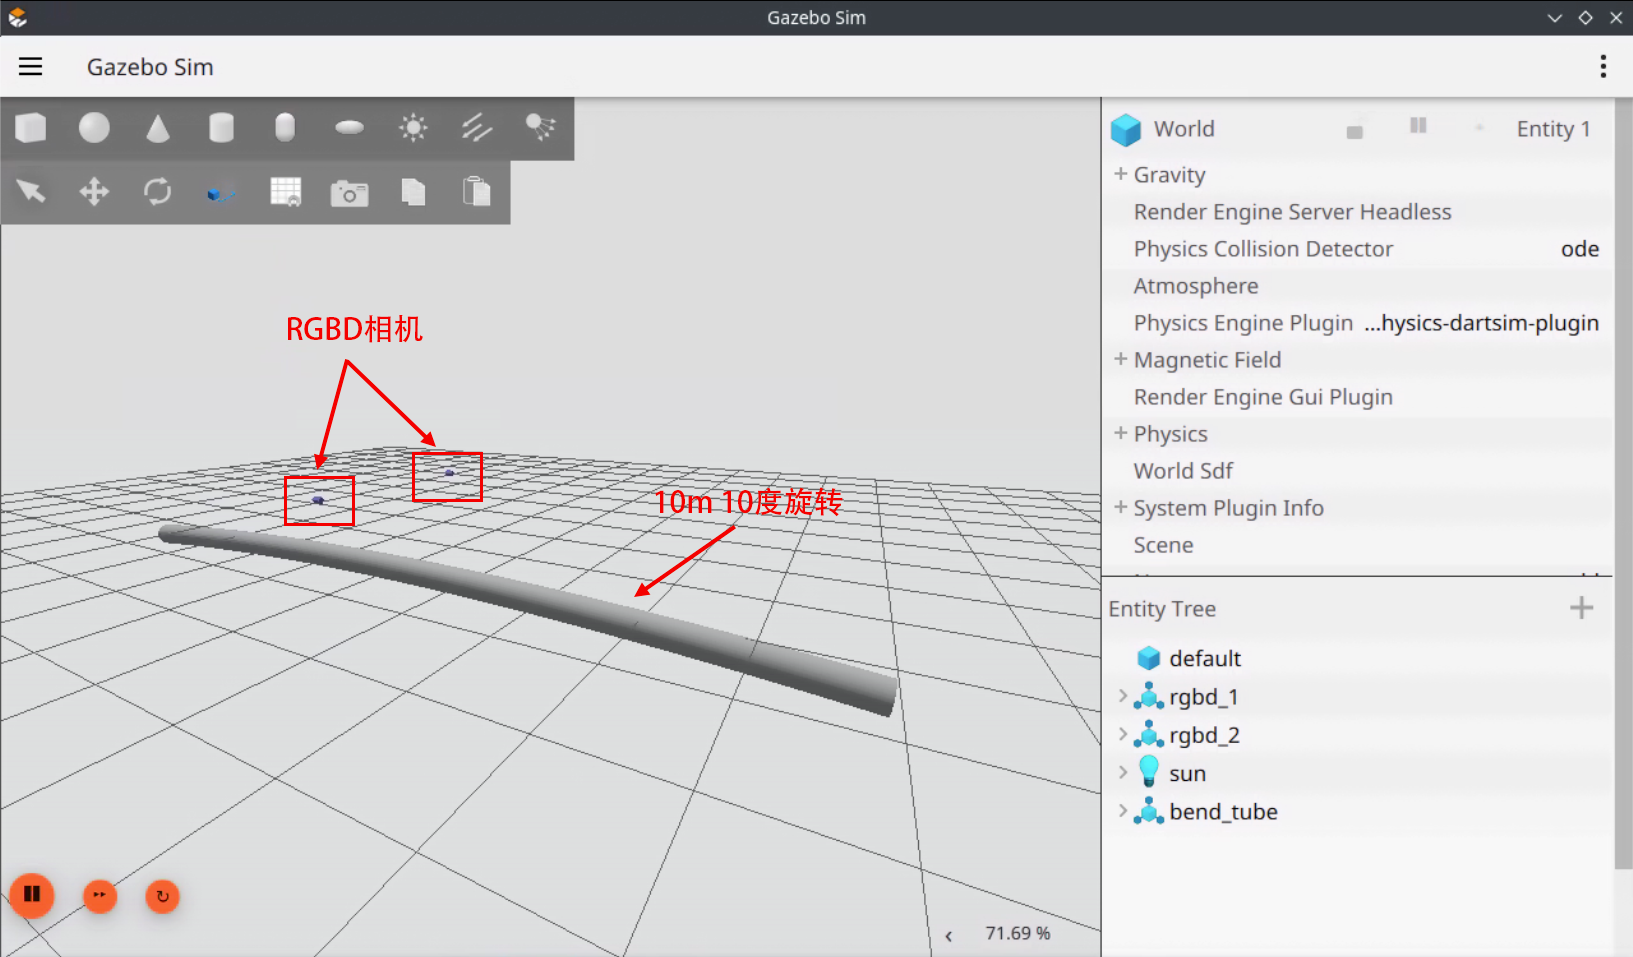
\includegraphics[width=0.8\linewidth]{images/sim_env.png}
    \caption{仿真环境示意}
    \label{fig:simulation_environment}
\end{figure}

为还原实际运行环境，在钢管匀速运行中，我们添加了低频振动和旋转位移扰动，
模拟传送带运行过程中可能出现的机械振动和安装误差及钢管在运动过程中横向滚动和旋转。
因此，仿真过程中，钢管运动的实际Z轴转角，Y-Z轴坐标变换如图\ref{fig:simulation_perturbation}所示。

\begin{figure}[!htb]
    \centering
    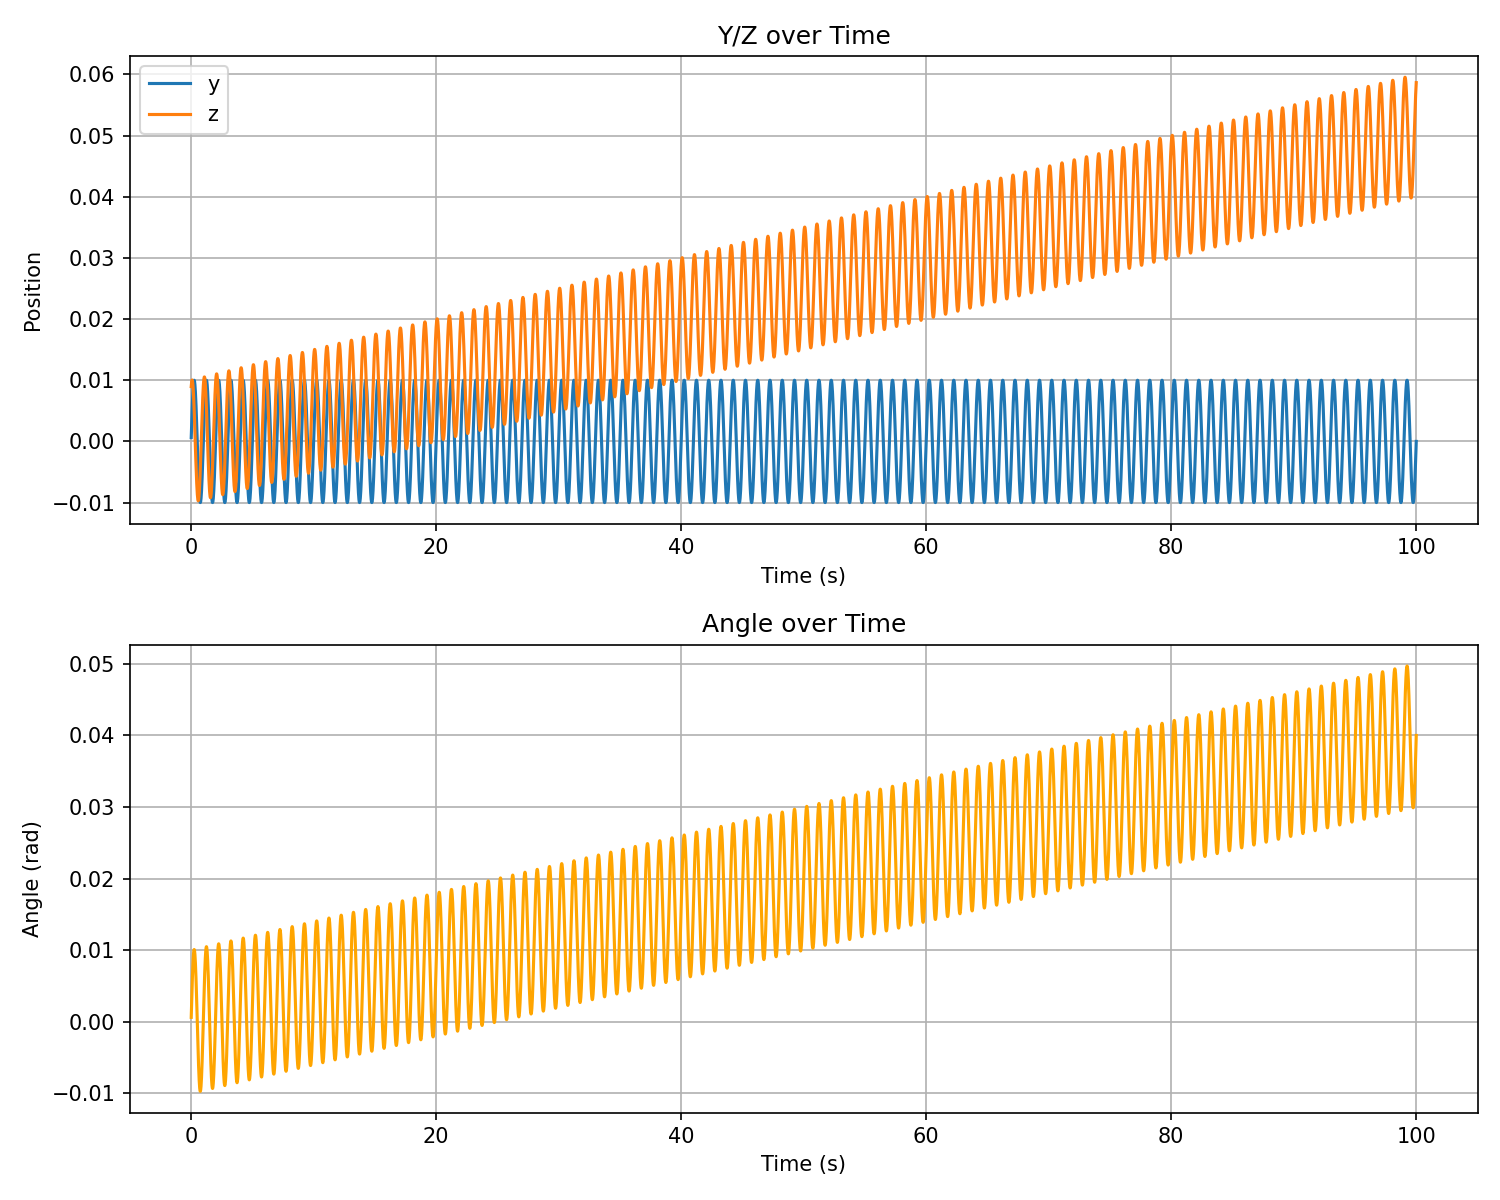
\includegraphics[width=0.8\linewidth]{images/pose_plot.png}
    \caption{仿真扰动示意}
    \label{fig:simulation_perturbation}
\end{figure}

仿真中使用的传感器参数如表\ref{tab:sensor_params}所示，各类噪声的形式与幅值如表\ref{tab:noise_summary}所示。

\begin{table}[!htb]
    \centering
    \caption{RGBD传感器参数}
    \label{tab:sensor_params}
    \begin{tabular}{ll}
        \toprule
        参数 & 值 \\
        \midrule
        分辨率 & 848$\times$480 \\
        水平FOV & 1.047\,rad（60°）\\
        帧率 & 10\,Hz \\
        深度范围 & 0.1$\sim$2.0\,m \\
        安装位置 & $y=\pm1.0$\,m，$z=1.0$\,m，45°斜向内俯视 \\
        \bottomrule
    \end{tabular}
\end{table}

\begin{table}[!htb]
    \centering
    \caption{噪声来源汇总}
    \label{tab:noise_summary}
    \begin{tabular}{llll}
        \toprule
        来源 & 形式 & 幅值 & 频率/规律 \\
        \midrule
        深度相机测距噪声 & 高斯，零均值 & $\sigma=0.002$\,m & 每帧独立 \\
        钢管平移振动（$y/z$） & 正弦，零均值 & 0.01\,m & 1.0\,Hz \\
        钢管角度振动（绕$z$轴） & 正弦，叠加在静态倾角上 & 0.01\,rad & 1.0\,Hz \\
        $z$方向缓变漂移 & 线性，随行程比例$t\in[0,1]$ & 0$\sim$0.05\,m & 单程 \\
        角度缓变漂移（绕$z$轴） & 线性，随行程比例$t\in[0,1]$ & 0$\sim$0.04\,rad & 单程 \\
        \bottomrule
    \end{tabular}
\end{table}

\section{测试平台设计}

\subsection{微缩测试架设计}
为验证本团队提出的非接触式钢管直线度检测方案的可行性，研发了本套钢管直度检测实验装置。
该装置采用非移动式设计理念，将待检测钢管固定于装置中央，通过驱动相机沿钢管轴向自动扫描，
实现全自动化数据采集，消除人工采集引入的粗大误差，为后续算法验证提供稳定、可靠的数据源。

\subsubsection{设计目标和装置参数}

本装置的核心设计目标为：在钢管完全固定的条件下，驱动深度相机沿轴向匀速扫描，连续采集钢管表面三维深度信息。
主要技术指标如下：

\begin{itemize}
    \item 线性采集速度可调，速度误差不超过$\pm5\%$
    \item 整机重量不超过20\,kg
    \item 整机长度不超过待检测钢管长度的130\%
    \item 整机体积不超过待检测钢管体积的300\%
    \item 工作温度范围：$-10\,^\circ\text{C}$ 至 $45\,^\circ\text{C}$
    \item 所有部件具备可替换性，支持快速维护
\end{itemize}

检测对象为长度2000\,mm、外径200\,mm、壁厚2\,mm的仿真钢管模型。

\subsubsection{装置概述}

装置总体采用笼式结构布置，将待检测钢管置于装置中央。前端两侧固定驱动电机，右端两侧固定传动轴系，
中间安装直线滑轨及门式支架。传动方案采用”伺服电机+齿轮+同步带”，驱动安装有深度相机的门式支架
沿高精度直线导轨做双向匀速运动，实现对钢管外表面的自动化全覆盖扫描。
固定支架提供可靠的支撑与夹持，确保钢管在整个测量过程中位置固定。

\subsubsection{结构设计}

装置主体框架采用国标4040铝型材搭建，具备轻质、高强、耐腐蚀、易于加工与装配的优点，
适合快速构建实验原型设备。系统总体结构如图\ref{fig:mechanical_structure_overview}所示。

\begin{figure}[!htb]
	\centering
	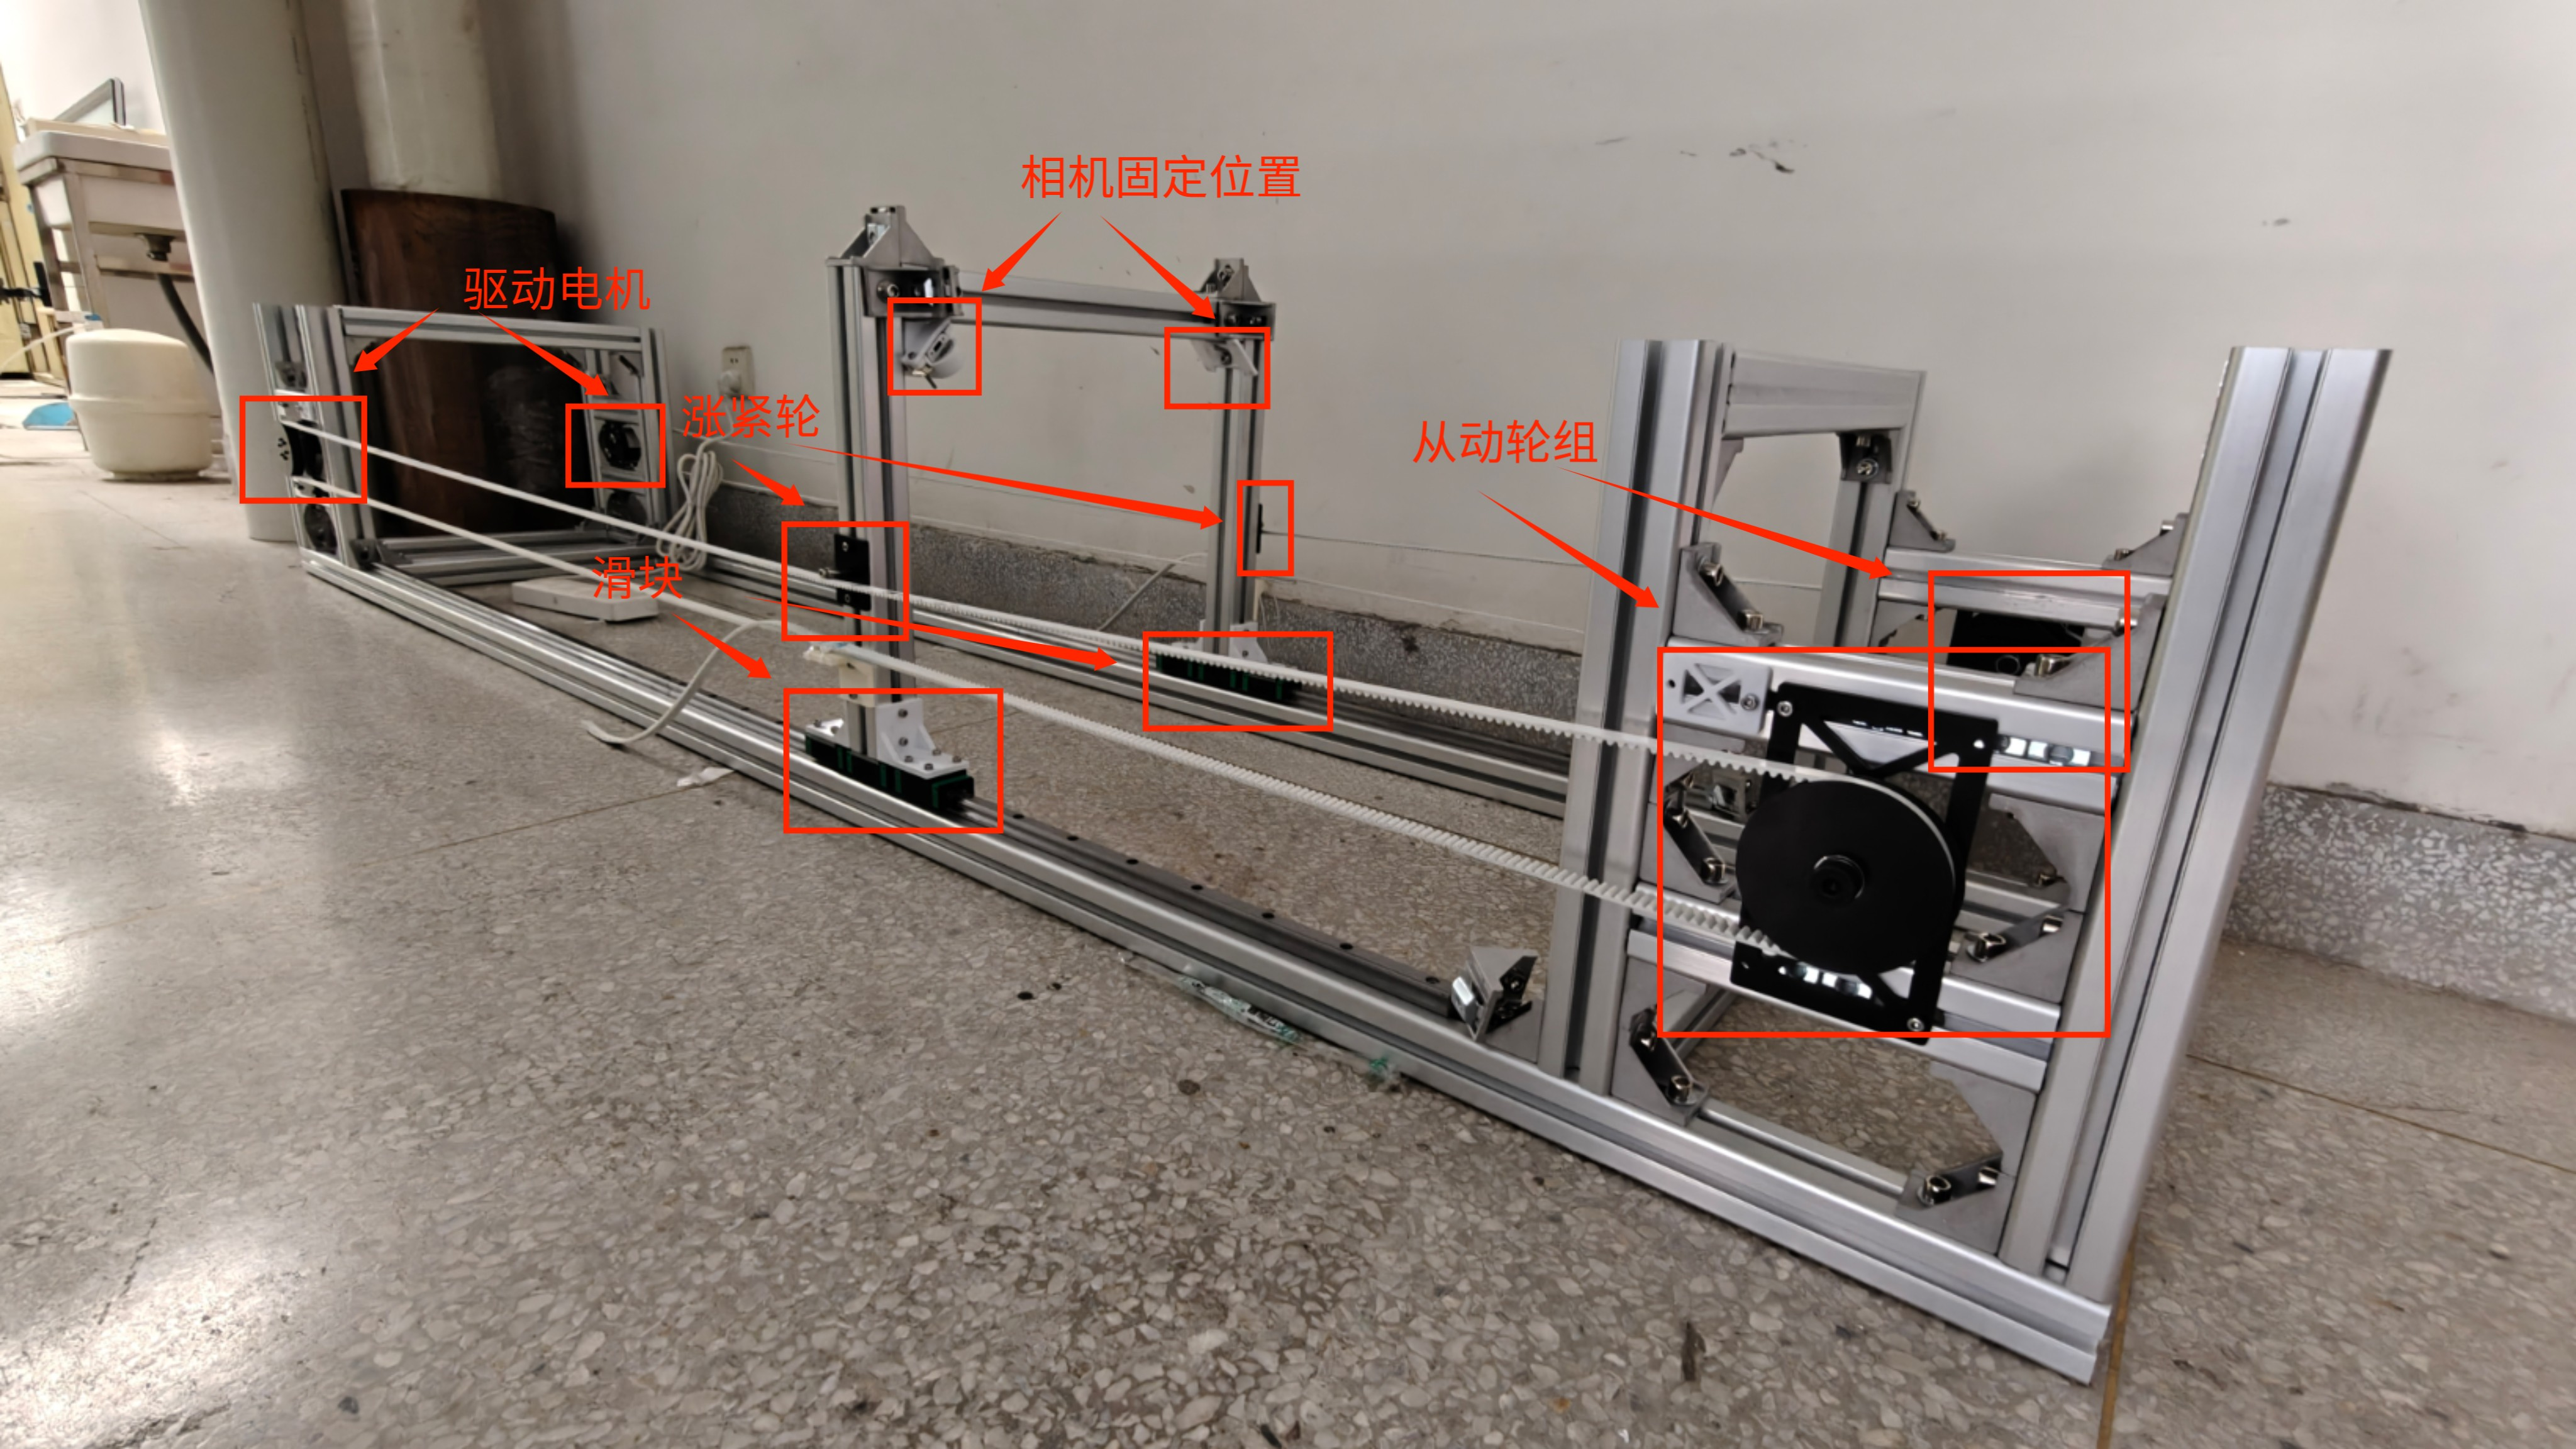
\includegraphics[width=\linewidth]{images/real_device.jpeg}
	\caption{机械结构总览}
	\label{fig:mechanical_structure_overview}
\end{figure}

装置主要由以下功能组件构成：
\begin{itemize}
\item 固定支架：如图\ref{fig:mechanical_structure_fixed_support}所示，采用V型块或定制夹具承载并锁紧仿真钢管模型，
      确保钢管在检测过程中无轴向移动或径向滚动。
\item 直线运动模块：包含高负载线性滑轨、滑块、同步带、驱动轮、从动轮及张紧机构。门式支架通过底部滑块连接在滑轨上，
      由同步带驱动实现精确的直线往复运动；传动带与门式支架、门式支架与滑块均采用螺纹连接。
      滑块部分如图\ref{fig:mechanical_structure_slide}所示。
\item 驱动单元：采用达秒4310伺服关节电机，最大扭矩输出5\,N$\cdot$m，控制误差在1°以内，
      通过专用电机安装板固定于铝型材框架端部。电机轴安装齿轮，经同步带将动力传递至门式支架，
      主控板通过PID控制对电流环及位置环进行实时控制，实现期望扫描速度。
\item 相机安装板：定制化安装板件，将两台Intel D435实感深度相机分别固定于门式支架左右内侧，
      相机光轴斜向下40°朝向待测钢管，确保对钢管表面的有效覆盖。
      板上设有调节机构，可微调相机高度和俯仰角度。
\end{itemize}

\begin{figure}[!htb]
	\centering
	\begin{subfigure}{0.48\textwidth}
		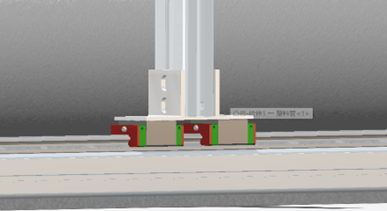
\includegraphics[width=\linewidth]{images/mechanical_structure_slide.png}
		\caption{滑台结构示意}
		\label{fig:mechanical_structure_slide}
	\end{subfigure}
	\hfill
	\begin{subfigure}{0.48\textwidth}
		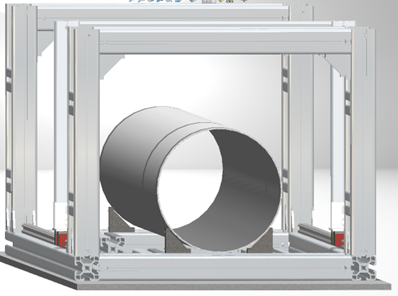
\includegraphics[width=\linewidth]{images/mechanical_structure_fixed_support.png}
		\caption{固定支撑结构示意}
		\label{fig:mechanical_structure_fixed_support}
	\end{subfigure}

	\caption{机械结构细节}
	\label{fig:mechanical_structure_details}
\end{figure}


\section{结论及讨论}

\subsection{结果}

基于仿真模型，我们对上述算法进行了验证，结果如图\ref{fig:results}所示。仿真钢管长度10\,m，弯曲角度10°。由于相机测量范围有限，仅保留可测量范围内的钢管局部点云进行计算，以均匀弯曲圆弧估计，理论端点间弓高约为0.1964\,m（圆弧半径$R = L/(2\sin5°) \approx 57.4$\,m，弓高$f = R(1-\cos5°) \approx 0.219$\,m，实际测量段较短，取局部有效段对应弓高0.1964\,m）。

\begin{figure}[!htb]
    \centering
    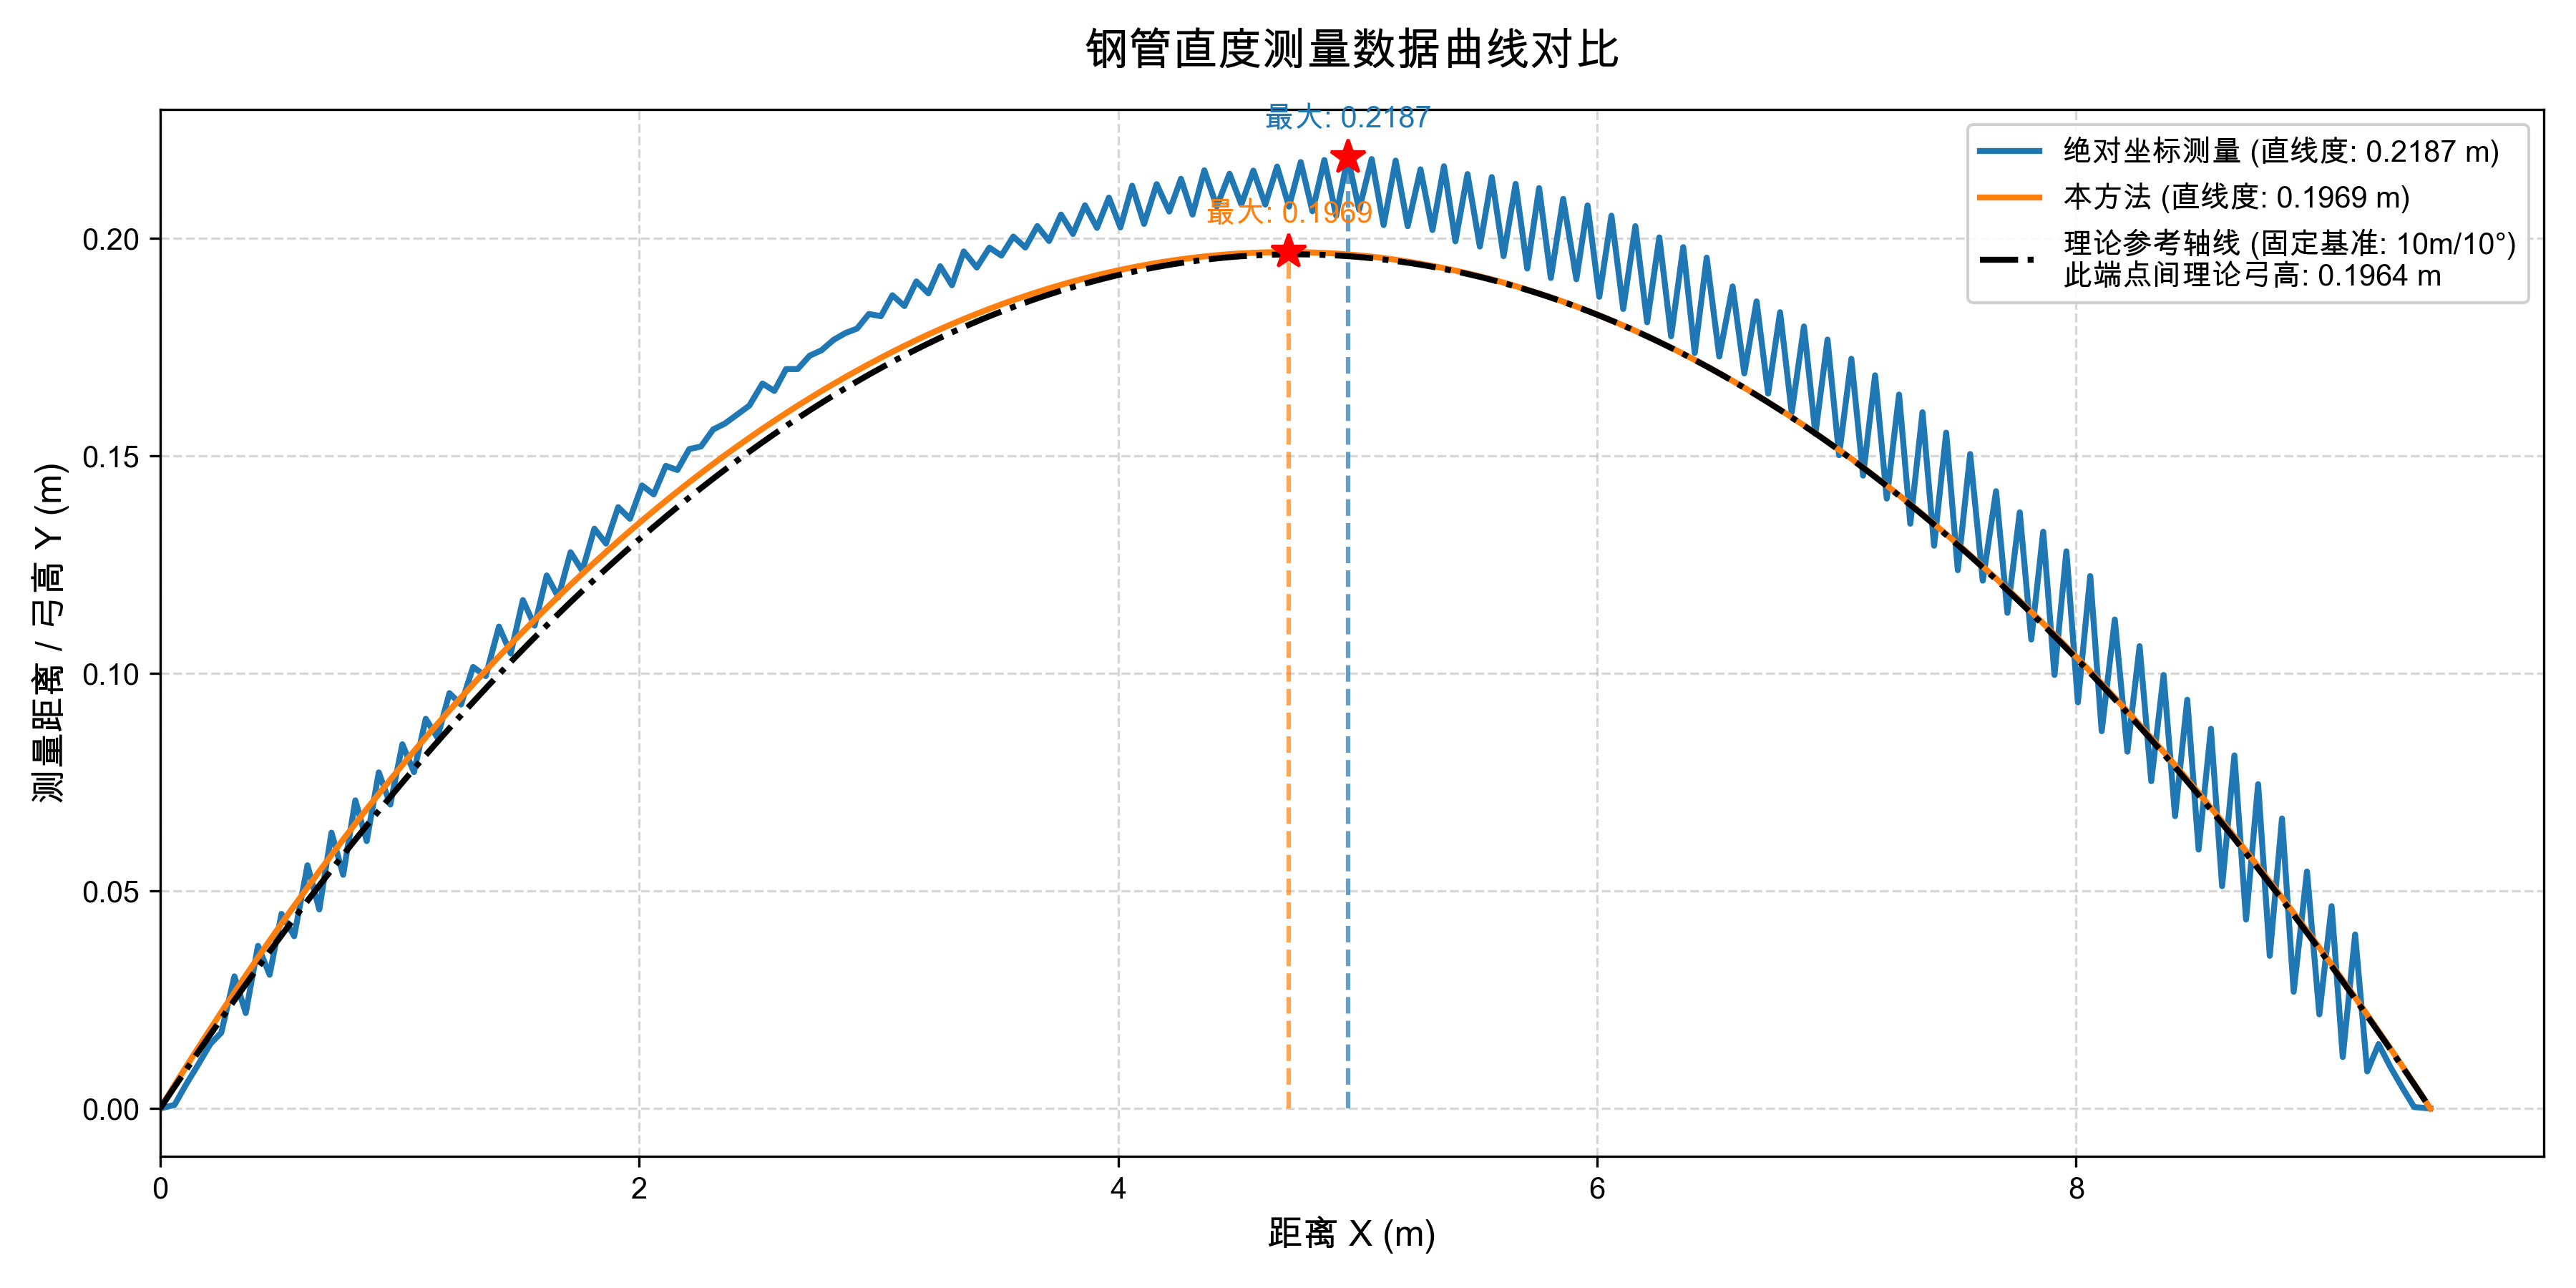
\includegraphics[width=\linewidth]{images/straightness_plot_fixed_radius.png}
    \caption{钢管直度测量数据曲线对比}
    \label{fig:results}
\end{figure}

在添加了振动和位移扰动（见表\ref{tab:noise_summary}）的情况下，绝对坐标法测得直度为0.2187\,m，相对理论值偏差11.4\%；本方法通过二阶差分消除刚体运动误差后，测得直度为0.1969\,m，相对理论值偏差仅0.3\%，误差降低约97\%。从曲线形态可以看出，绝对坐标法受振动扰动影响产生明显高频波动，而本方法输出曲线与理论参考轴线高度吻合，有效抑制了钢管轴向进给过程中位移抖动对测量精度的影响。

\subsection{不足之处}

本系统在以下几个方面存在明显局限：

\textbf{主弯曲方向假设。}算法依赖"钢管存在某一弯曲方向曲率远大于其他方向"的前提，通过加权PCA将三维问题降为二维处理。若钢管在多个方向存在相近幅值的弯曲，主弯曲平面提取将失准，导致直度计算结果偏低。

\textbf{螺旋扭曲假设。}算法假设钢管沿轴向的螺旋扭曲较轻微，即各截面的截面坐标系方向变化缓慢。若钢管存在显著的螺旋扭曲，PCA轴线估计与圆拟合的截面方向将产生系统性偏差，影响圆心坐标精度。

\textbf{头尾端处理不足。}二阶差分法需要三点才能计算一个曲率值，导致钢管首尾各一个切片位置无法直接获得曲率估计。此外，两次数值积分在边界处缺乏约束，积分漂移在头尾端最为显著，直度计算对端部数据较为敏感。

\textbf{依赖精确位置传感器。}分Bin操作和截面绝对坐标计算均依赖传送带位置传感器提供准确的轴向位移数据。若编码器存在累积误差或打滑，各截面的轴向坐标将产生偏移，导致Bin分配错误和轴线重建失真。

\textbf{传感器精度有限。}系统采用Intel D435消费级RGBD相机，深度测量噪声约为$\sigma \approx 2\,\text{mm}$，远高于工业直度检测的亚毫米级精度要求。在当前硬件条件下，算法的理论精度上限受限于传感器本身，测试结果仅具参考意义。

\textbf{实物验证未按期完成。}受限于开发进度，圆拟合、二阶差分、分Bin平均及曲率积分等核心算法均未在真实硬件平台上完成端到端验证，目前仅完成了点云分割算法的实物验证。

\begin{thebibliography}{99}
	\bibitem{cv} Lu, R. S., Li, Y. F., \& Yu, Q. (2001). On-line measurement of the straightness of seamless steel pipes using machine vision technique. \textit{Sensors and Actuators A: Physical}, \textit{94}(1--2), 95--101.
	\bibitem{pm} Gao, W., Yokoyama, J., Kojima, H., \& Kiyono, S. (2002). Precision measurement of cylinder straightness using a scanning multi-probe system. \textit{Precision Engineering}, \textit{26}(3), 279--288.
	\bibitem{hxf} 黄雄飞, 张乾峰, 张全宝, 等. (2017). 直缝钢管直度测量方法的探讨. \textit{焊管}, \textit{40}(5), 41--43.
	\bibitem{pca} Hotelling, H. (1933). Analysis of a complex of statistical variables into principal components. \textit{Journal of Educational Psychology}, \textit{24}(6), 417--441. https://doi.org/10.1037/h0071325
	\bibitem{ransac} Fischler, M. A., \& Bolles, R. C. (1987). Random sample consensus: A paradigm for model fitting with applications to image analysis and automated cartography. In M. A. Fischler \& O. Firschein (Eds.), \textit{Readings in Computer Vision} (pp. 726--740). Morgan Kaufmann. https://doi.org/10.1016/B978-0-08-051581-6.50070-2
	\bibitem{wpca} Fan, Z., Liu, E., \& Xu, B. (2011). Weighted principal component analysis. In \textit{Proceedings of the Third International Conference on Artificial Intelligence and Computational Intelligence (AICI'11)} (pp. 569--574). Springer-Verlag.
	\bibitem{aniso} Corona, E., Lee, L.-H., \& Kyriakides, S. (2006). Yield anisotropy effects on buckling of circular tubes under bending. \textit{International Journal of Solids and Structures}, \textit{43}(22), 7099--7118. https://doi.org/10.1016/j.ijsolstr.2006.03.005
	\bibitem{cv_yd} Kshaurad, K., Kiran, M. B., \& Shanmuganatan, S. P. (2021). Minimum zone tolerance algorithm to detect roundness error for machined rods using vision system. \textit{Materials Today: Proceedings}, \textit{46}, 5997--6003. https://doi.org/10.1016/j.matpr.2020.12.788
	\bibitem{tzzxd} Egidi, A., Balsamo, A., Corona, D., \& Pisani, M. (2023). Investigation on modulation-based straightness measurement. \textit{Sensors}, \textit{23}(6), 2912. https://doi.org/10.3390/s23062912
\end{thebibliography}

\end{document}
